\documentclass[11pt]{article}
\usepackage{graphicx}
\usepackage{lscape}
\usepackage{pdfpages}
\usepackage{scrextend}
\usepackage{gensymb}
\usepackage{subcaption}
\usepackage{rotating}
\usepackage[titletoc]{appendix}
\usepackage{setspace}
\usepackage{caption, float, multirow}

\setlength{\oddsidemargin}{0.3in}
\setlength{\textwidth}{5.9in}
\setlength{\topmargin}{-0.4in}
\setlength{\textheight}{8.5in}

\makeatletter
    \setlength\@fptop{0\p@}
\makeatother

\begin{document}

\doublespacing

\title{\textbf{ME533 -- Applicability of the Composite Rule-of-Mixtures for the Description of the Mechanical Properties of PBT Polymeric Matrix-Short Glass Fiber System}}
\author{Alan Wu, Jan Quijalvo, Ryan Lam}
\date{\today}


\makeatletter
    \singlespacing
    \begin{titlepage}
        \begin{center}
        	\begin{figure}[h]
        	\centering
            
\includegraphics[scale=0.3]{./figures/University-of-Waterloo}
            \end{figure}
            \vspace{20mm}
            {\huge \bfseries  \@title }\\[2ex] 
            \vspace{5mm}
            {\LARGE Alan Wu}\\
            \vspace{2mm}
            {\LARGE Jan Quijalvo}\\
            \vspace{2mm}
            {\LARGE Ryan Lam}\\
            \vspace{2mm}
            \LARGE 4B Mechanical Engineering\\[12ex]
            Prepared for\\
            ME 533 - Composite Materials with Non-metallic and Metallic Matrices\\
            Robert A. Varin
            \centering
            \vfill
            {\large April 3, 2017}
        \end{center}
    \end{titlepage}
\makeatother

\tableofcontents
\newpage
\listoffigures
\newpage
\listoftables
\newpage

\section{Introduction}
This lab is meant to blah blah

\section{Experimental Procedure}
This is how we do.

\section{Results}
From conducting the experiment and examining the microstructures of each of the composities (PBT12, PBT11, and PBT14), the following microstructural properties can be found. Since PBT14 had no fibers, these values are not applicable for it.

\begin{itemize}
\item Average volume fraction of reinforcing fibers
\item Average length of the fibers
\item Average diameter of the fibers
\item Average aspect ratio
\item Volume fraction of matrix
\item Volume fraction of voids (qualitative)
\end{itemize}

These values were determined by counting and measuring fiber lengths and diameters seen under the microscope and averaging the greatest 20 results. Figures \ref{pbt11longcount}, \ref{pbt11transcount}, \ref{pbt12longcount}, and \ref{pbt12transcount} show how this was done. In both samples, the fibers were counted and measured in various places around the sample area. For the longitudinal fibers, only fully revealed fibers were counted (rectangular ends). The volume fractions for the samples of PBT11 and PBT12 were calculated by determining the ratio of the cross-sectional area of the transverse fibers in the field of view of the microscope to the field of view of the microscope.

\begin{figure}[H]
\centering
\includegraphics[width=.7\linewidth]{figures/PBT11_Long.png}
\caption{PBT11 Longitudinal Fiber Counting}
\label{pbt11longcount}
\end{figure}
\begin{figure}[H]
\centering
\includegraphics[width=.7\linewidth]{figures/PBT11_Trans.png}
\caption{PBT11 Transverse Fiber Counting}
\label{pbt11transcount}
\end{figure}
\begin{figure}[H]
\centering
\includegraphics[width=.7\linewidth]{figures/PBT12_Long.png}
\caption{PBT12 Longitudinal Fiber Counting}
\label{pbt12longcount}
\end{figure}
\begin{figure}[H]
\centering
\includegraphics[width=.7\linewidth]{figures/PBT-12-TRANSVERSE-COMBINED.png}
\caption{PBT12 Transverse Fiber Counting}
\label{pbt12transcount}
\end{figure}

The following table lists the respective values for PBT9, PBT11, PBT12, and PBT14. For PBT9 it was assumed that the fibers used in the composite would be the same as PBT11 and PBT12. The fiber lengths and diameters were simply calculated as the respective average of the same values for PBT11 and PBT12.
Since PBT14 had no fibers in the polymer, these values were ignored, or set to zero.
\onehalfspacing
\begin{center}
\captionof{table}{PBT9, PBT11, PBT12, and PBT14 Values} \label{tab:MeasuredValues}
\begin{tabular}{p{1.5cm} || p{2.cm} | p{2.cm} | p{2.cm} | p{2.cm}}
\hline
Sample & \multicolumn{1}{c|}{PBT9} & \multicolumn{1}{c|}{PBT11} & \multicolumn{1}{c|}{PBT12} & \multicolumn{1}{c}{PBT14} \\
\hline
\hline
\(V_f\) & 0.224 & 0.179 & 0.135 & 0\\
\(\ell (\mu m)\) & 294.14 & 299.33 & 288.94 & N/A\\
\(d (\mu m) \) & 14.61 & 14.60 & 14.61 & N/A\\
\(\ell /d\) & 20.14 & 20.50 & 19.77 & N/A\\
\(V_m\) & 0.78 & 0.82 & 0.86 & 1 \\
\(V_v\) & Less & Less & Many & Many\\
\hline
\end{tabular}
\end{center}
\singlespacing
\vspace{1em}

Table \ref{tab:MaterialValues} shows the mechanical material properties of the fiber (E-Glass) and matrix (PBT) materials. 

\onehalfspacing
\begin{center}
\captionof{table}{Material Data for E-Glass Fiber and PBT Polymer} \label{tab:MaterialValues}
\begin{tabular}{p{2cm} || p{2.75cm} | p{2.75cm} | p{2.75cm} }
\hline
\multicolumn{1}{c||}{Material} & Young's Modulus (MPa) & \(\sigma^*\), Fracture Strength (MPa) & Shear Modulus (MPa) \\
\hline
\hline
\(E-Glass\) & 70000 &  1750 & 881.6 \\
\(PBT\) & 2558 & 32.467 & N/A\\
\hline
\end{tabular}
\end{center}
\singlespacing
\vspace{1em}


The following figures show tensile tests performed for samples of PBT9, PBT11, PBT12, and PBT14 in the elastic regions and up to fracture.
\\
\begin{figure}[H]
\centering
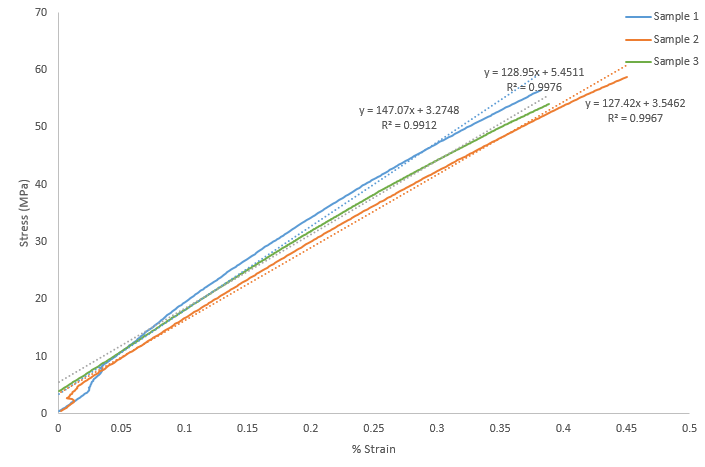
\includegraphics[width=.95\linewidth]{figures/PBT9_Tensile.png}
\caption{PBT9 Tensile Test}
\label{pbt9tensile}
\end{figure}

\begin{figure}[H]
\centering
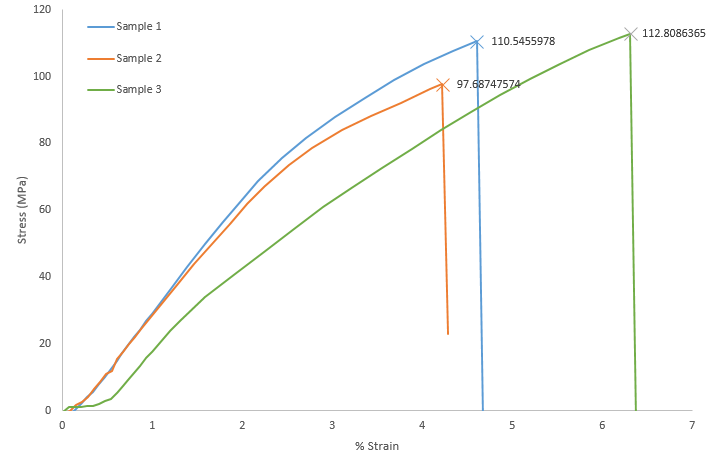
\includegraphics[width=.95\linewidth]{figures/PBT9_Fail.png}
\caption{PBT9 Test to Failure}
\label{pbt9fail}
\end{figure}

\begin{figure}[H]
\centering
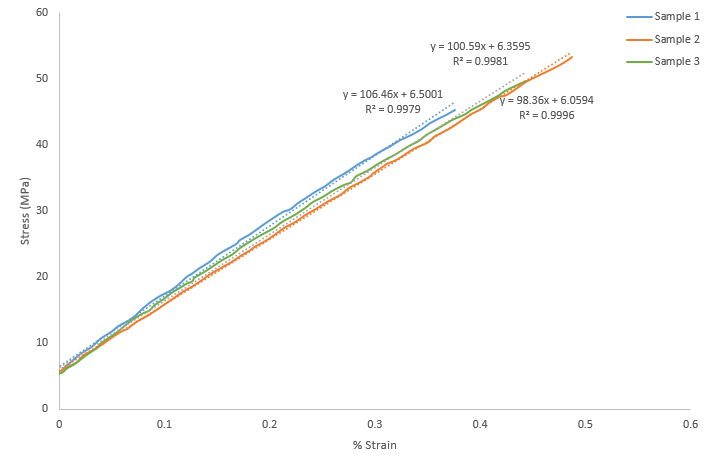
\includegraphics[width=.95\linewidth]{figures/PBT11_Tensile.png}
\caption{PBT11 Tensile Test}
\label{pbt11tensile}
\end{figure}

\begin{figure}[H]
\centering
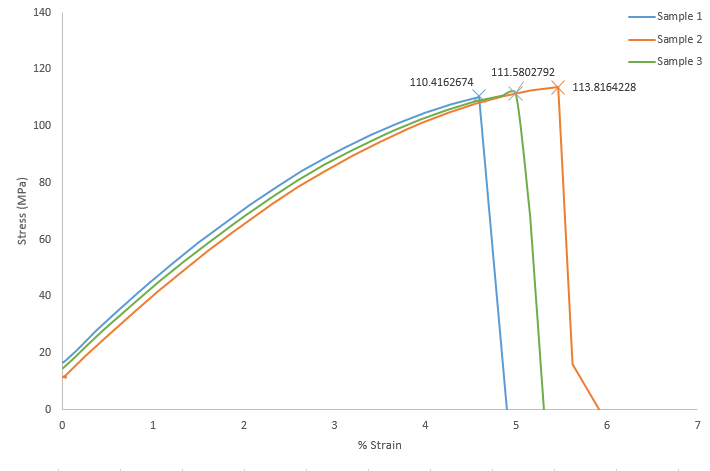
\includegraphics[width=.95\linewidth]{figures/PBT11_Fail.png}
\caption{PBT11 Test to Failure}
\label{pbt11fail}
\end{figure}

\begin{figure}[H]
\centering
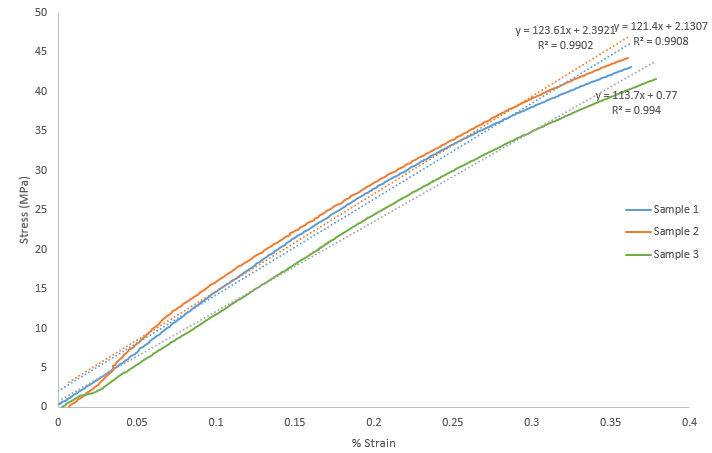
\includegraphics[width=.95\linewidth]{figures/PBT12_Tensile.png}
\caption{PBT12 Tensile Test}
\label{pbt12tensile}
\end{figure}

\begin{figure}[H]
\centering
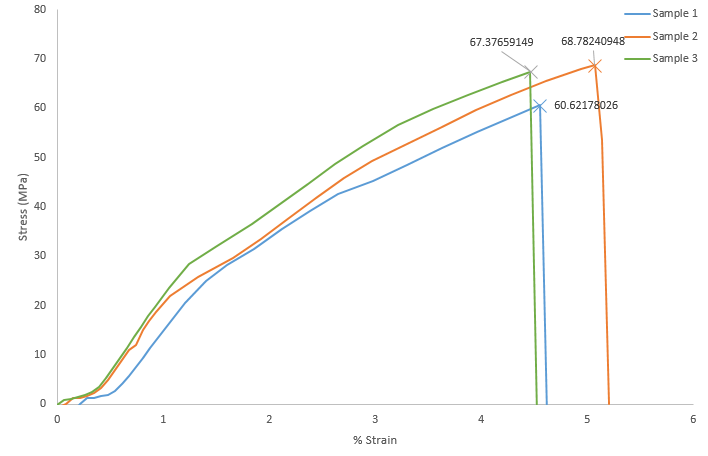
\includegraphics[width=.95\linewidth]{figures/PBT12_Fail.png}
\caption{PBT12 Test to Failure}
\label{pbt12fail}
\end{figure}



\begin{figure}[H]
\centering
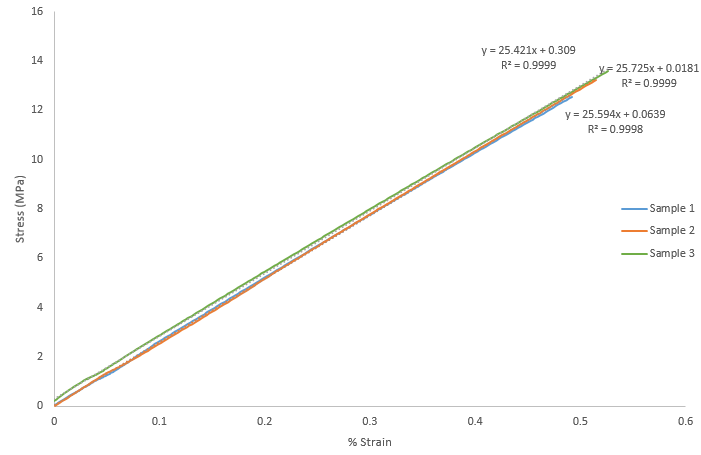
\includegraphics[width=.95\linewidth]{figures/PBT14_Tensile.png}
\caption{PBT14 Tensile Test}
\label{pbt14tensile}
\end{figure}

\begin{figure}[H]
\centering
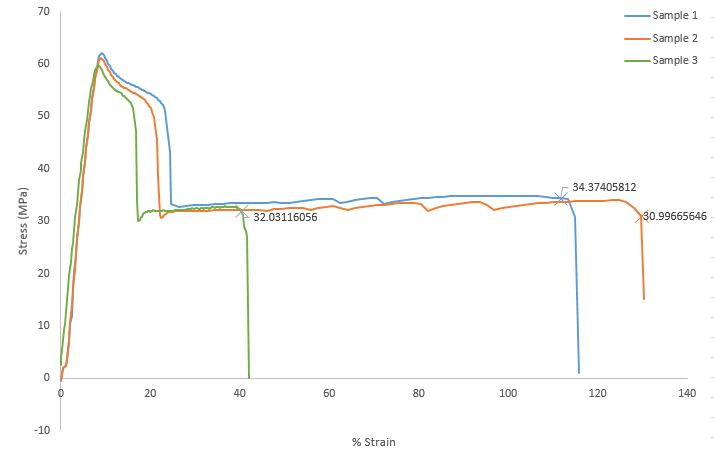
\includegraphics[width=.95\linewidth]{figures/PBT14_Fail.png}
\caption{PBT14 Test to Failure}
\label{pbt14fail}
\end{figure}

\newpage
\section{Discussion}


Using the values in Table \ref{tab:MeasuredValues} and Table \ref{tab:MaterialValues} the elastic modulus of the samples can be found using both the Halpin approach (Equation \ref{eq:halpin}) and simple equation (Equation \ref{eq:simple}). First, it is helpful to determine which set of equations are valid for this case. This requires the \textit{critical fiber length}, \(\ell_c\), calculated using the following.

\begin{equation}
\ell_c = \frac{\sigma^*_f r}{\tau^*_i}
\end{equation}
\\

The \textit{critical fiber length} for the PBT samples are approximately 787 microns, and since the average fiber lengths found in the samples (Table \ref{tab:MeasuredValues})0[ are lower than the critical length, it is valid to use the short fiber equations.

\begin{equation} \label{eq:halpin}
\frac{E^{short}_{\downarrow \downarrow}}{E_m} = \frac{1+\xi \eta V_f}{1-\eta V_f}
\end{equation}

To calculate \(E_{\downarrow \downarrow}^{short}\) using the Halpin method, two variables are required, \(\eta\) and \(\xi\), which are calculated using the following:

\begin{equation}
\eta = \frac{E_f/E_m-1}{E_f/E_m+\xi}
\end{equation}

\begin{equation}
\xi = 2 \frac{l}{d} +40V^{10}_f
\end{equation}
\\
The simple method of calculating \(E_{\downarrow \downarrow}^{short}\) is shown in the following equation.

\begin{equation} \label{eq:simple}
E^{short}_{\downarrow \downarrow} = \eta_l E_f V_f + E_m(1-V_f)
\end{equation}

This method requires the calculation of a \textit{length correction factor}, \(\eta_l\), found using the following equation.

\begin{equation}
\eta_l = 1- \left[\frac{\tanh 0.5\beta l}{0.5\beta l} \right]
\end{equation}

\begin{equation}
\beta=\left[\frac{2G_m}{E_fr^2 ln(\frac{R}{r})}\right]^{1/2}
\end{equation}
\\
The fracture stress of the composites were also calculated using Equation \ref{eq:fracture}.
 
\begin{equation} \label{eq:fracture}
\sigma^*_{\downarrow \downarrow} = \left( \frac{l}{2l_c}\right) \sigma_f^* V_f + \sigma^*_m V_m
\end{equation}


The results of these calculations are shown in the following table.
\\
\onehalfspacing
\begin{center}
\captionof{table}{PBT9, PBT11, PBT12, and PBT14 Modulus and Fracture Stress} \label{tab:CalculatedValues}
\begin{tabular}{p{3.5cm} || p{2.cm} | p{2.cm} | p{2.cm} | p{2.cm}}
\hline
Sample & \multicolumn{1}{c|}{PBT9} & \multicolumn{1}{c|}{PBT11} & \multicolumn{1}{c|}{PBT12} & \multicolumn{1}{c}{PBT14} \\
\hline
\hline
\(E^{short}_{\downarrow \downarrow}\) Halpin (MPa)& 12658.3 &  10508.06 & 8376.91 & 2558\\
\(E^{short}_{\downarrow \downarrow}\) Simple (MPa)& 12256.6 & 10366.57 & 8338.3 & 2558\\
\(\sigma^*_{\downarrow \downarrow}\) (MPa)& 98.42 & 86.12 & 71.37 & 32.47\\
\(\ell_c (\mu m) \) & 787.31 & 787.65 & 787.65 & N/A\\
\hline
\end{tabular}
\end{center}
\singlespacing

Comparing the results of these tensile tests to the analytical data in Table \ref{tab:CalculatedValues}, it is clear that there is some degree of error between the experimental and analytical results for PBT11 and PBT12. It was previously when doing the experiment that the tensile test for PBT12 was done incorrectly, leading to erroneous values for determining the Young's Modulus.

\onehalfspacing
\begin{center}
\captionof{table}{Tensile Test Data} \label{tab:ComparingValues}
\begin{tabular}{p{1.25cm} || p{1.5cm} | p{1.5cm} | p{1.5cm} | p{1.5cm} | p{1.5cm} | p{1.5cm} | p{1cm}}
\hline
 \multirow{2}{*}{Sample} & \multicolumn{3}{c|}{Young's Modulus (MPa)}  & 
   \multicolumn{3}{c|}{Fracture Stress (MPa)} & \multirow{2}{*}{\(V_f\)} \\
   & \multicolumn{1}{c}{Test} & \multicolumn{1}{c}{Calculated} & \multicolumn{1}{c|}{\% Error} & \multicolumn{1}{c}{Test} & \multicolumn{1}{c}{Calculated} & \multicolumn{1}{c|}{\% Error} &\\
\hline
PBT9 & 13448 & 12658.33 & 6.24 & 107.01 & 98.42 & 8.73 & 0.224\\
PBT11 & 10180.33 & 10508.06 & 3.12 & 111.94 & 86.12 & 29.97 & 0.179\\
PBT12 & 11957 & 8376.91 & 42.74 & 65.31 & 71.36 & 8.09 & 0.135 \\
PBT14 & 2558 & 2558 & 0 & 32.47 & 32.47 & 0 & 0\\
\hline
\end{tabular}
\end{center}
\singlespacing

Plotting the measured and calculated values of the Young's Modulus and the Fracture Stress helps to exemplify the differences between the experimental and analytical results, as shown in Figures \ref{FScompare} and \ref{ModulusCompare}.

\begin{figure}[H]
\centering
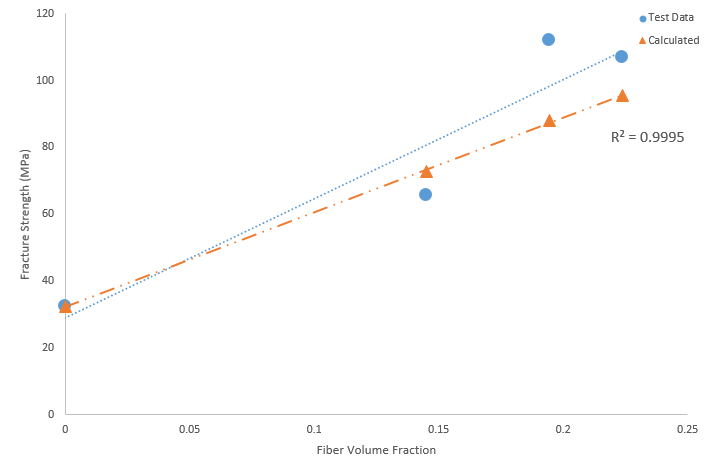
\includegraphics[width=.95\linewidth]{figures/fracture_stress_test_vs_calc.png}
\caption{Fracture Stress, Experimental vs. Analytical}
\label{FScompare}
\end{figure}

\begin{figure}[H]
\centering
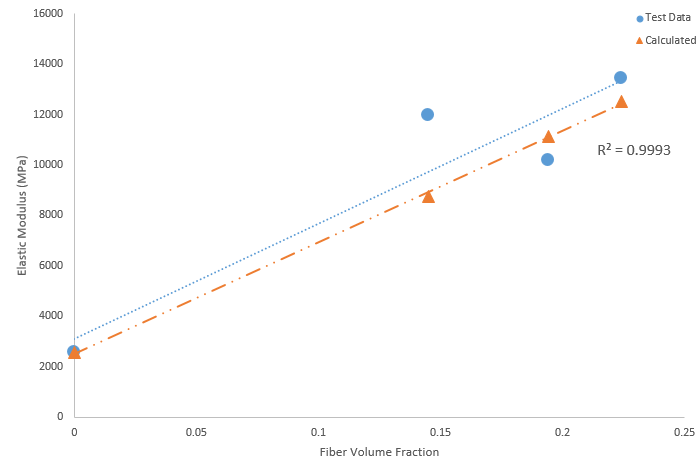
\includegraphics[width=.95\linewidth]{figures/modulus_test_vs_calc.png}
\caption{Young's Modulus, Experimental vs. Analytical}
\label{ModulusCompare}
\end{figure}

As mentioned before the test for PBT12 lead to erroneous results for the tested Young's Modulus value. Therefore, PBT12 has the largest error of 36.44\%. The rest of the calculated values for PBT9 and PBT11 are within a 10\% error and yield results close to the tested values. It can be seen from Figure \ref{FScompare} that as you go from PBT14 which contains no fibers to PBT12, 11 and  9, the Young's Modulus increases. This is attributed to the increasing volume fraction of E-Glass fibers. This can be predicted from the relationship in Equation \ref{eq:simple} for the calculation of Young's Modulus using the simple approach. The tested values should also show the same trend as the calculated values, but again, because of the error with testing PBT12, it shows a higher Young's Modulus than that of PBT11 which is not to be expected. This trend is plotted in Figure \ref{FScompare}.
\singlespacing

In terms of Fracture Strength, the different between the calculated and tested values is within 15\%. The main source of error is with PBT11. It displays a higher Fracture Strength than that of PBT9. From the relationship given by Equation \ref{eq:fracture}, the trend should be an increasing Fracture Strength with increasing volume fraction of fiber. SHIT THERE MIGHT BE LIKE... A LIMIT OR SOME SHIT.


\section{Conclusion}
We did some stuff using some PBT samples for the sake of testing some stuff. From testing and analysis we learned that something about the PBT or composites and we got these results. From this we can say that blah blah blah or something. 

\newpage
\begin{thebibliography}{9}
\bibitem{proposal} 
Ryan Lam, Jan Quijalvo, Robert Weeks and Alan Wu. 
Design Project Proposal. 
Unpublished manuscript, University of Waterloo, 2016.

\bibitem{asphaltAugerPic}
Engineering Control Guidelines for Hot Mix Asphalt Pavers. (2014). Retrieved July 26, 2016, from https://www.cdc.gov/niosh/docs/97-105/

\end{thebibliography}
\end{document}
